\documentclass{article}

\usepackage{amsmath}
\usepackage{minted}
\usepackage{graphicx}
\usepackage{caption}
\usepackage{subcaption}
\usepackage{mathrsfs}
\usepackage[toc,page]{appendix}

%Section style
\usepackage{etoolbox} %for configuration of sloppy
\usepackage{xcolor}


\definecolor{secnum}{RGB}{102,102,102}

\makeatletter
    \def\@seccntformat#1{\llap{\color{secnum}\csname the#1\endcsname\hskip 16pt}}
\makeatother
%end section style

\begin{document}

\section{I.2}

\subsection{I.2.1}

We are using the guassian function:
\begin{equation}
    f(x) = a * exp\left(-\frac{(x-b)^2}{2c^2}\right)
\end{equation}
Where:
\begin{align*}
    a &= \frac{1}{\sigma \sqrt{2\pi}}\\
    b &= \mu\\
    c &= \sigma 
\end{align*}
Giving us the full equation:
\begin{equation}
    f(x) = \frac{1}{\sigma \sqrt{2\pi}} * exp\left(-\frac{(x-\mu)^2}{2\sigma^2}\right)
\end{equation}


\begin{figure}[!ht]
    \centering
    \begin{subfigure}[b]{0.4\textwidth}
        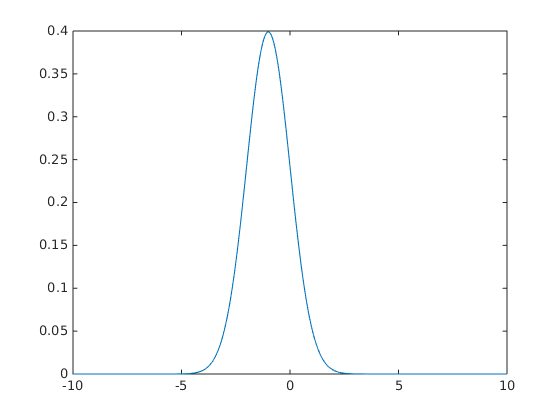
\includegraphics[width=\textwidth]{part1/I211.png}
        \caption{$(\mu, \sigma) = (-1,1)$}
    \end{subfigure}%
    \begin{subfigure}[b]{0.4\textwidth}
        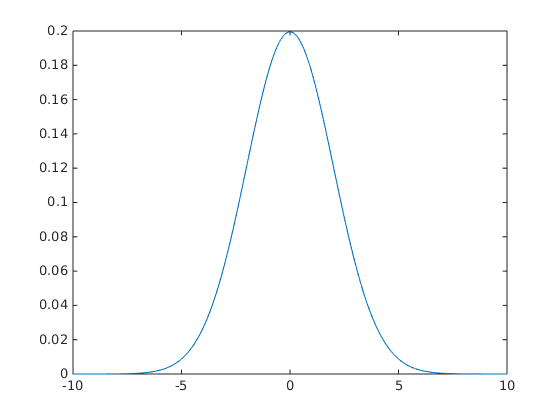
\includegraphics[width=\textwidth]{part1/I212.png}
        \caption{$(\mu, \sigma) = (0,2)$}
    \end{subfigure}
    \begin{subfigure}[b]{0.4\textwidth}
        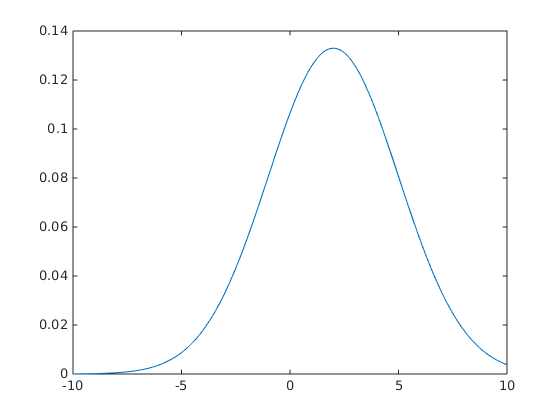
\includegraphics[width=\textwidth]{part1/I213.png}
        \caption{$(\mu, \sigma) = (2,3)$}
    \end{subfigure}
    \caption{Gaussian distribution with varying parameters}
    \label{fig:I1.1}
\end{figure}

\subsubsection{Code}

Using matlab we implemented (2) in the following code, giving us the
figures \ref{fig:I1.1}

\begin{minted}{matlab}
function [ f ] = gaussjohn( mu, sigma )
    a = 1 / (sigma * sqrt(2 * pi));
    f = @(x) a * exp(-((x - mu)^2) / (2 * sigma^2));
end

fplot(gaussjohn(-1,1), [-10,10])
fplot(gaussjohn( 0,2), [-10,10])
fplot(gaussjohn( 2,3), [-10,10])
\end{minted}

\subsection{I2.2}

We created two sets of normal distribution $\mathscr{N}(0,1)$, and extracted a sample with the distribution of $\mathscr{N}(y \| \mu, \sum)$ 
with mean:

\begin{equation}\label{eq:2.2mean}
    \mu = (1,2)^T
\end{equation} 
and covariance:

\begin{equation}\label{eq:2.2co}
    \sum = \left( \begin{array}{cc} 0.3 & 0.2 \\ 0.2 & 0.2 \end{array} \right)
\end{equation}
using the code seen below. This gave us the plots seen on Figure \ref{fig:I2.2}
\begin{figure}[!ht]
    \centering
    \begin{subfigure}[b]{0.5\textwidth}
        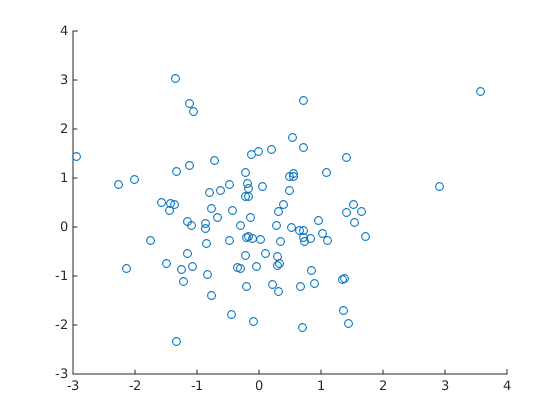
\includegraphics[width=\textwidth]{part1/I221.png}
        \caption{$\mathscr{N}(0,1)$ distribution}
    \end{subfigure}%
    \begin{subfigure}[b]{0.5\textwidth}
        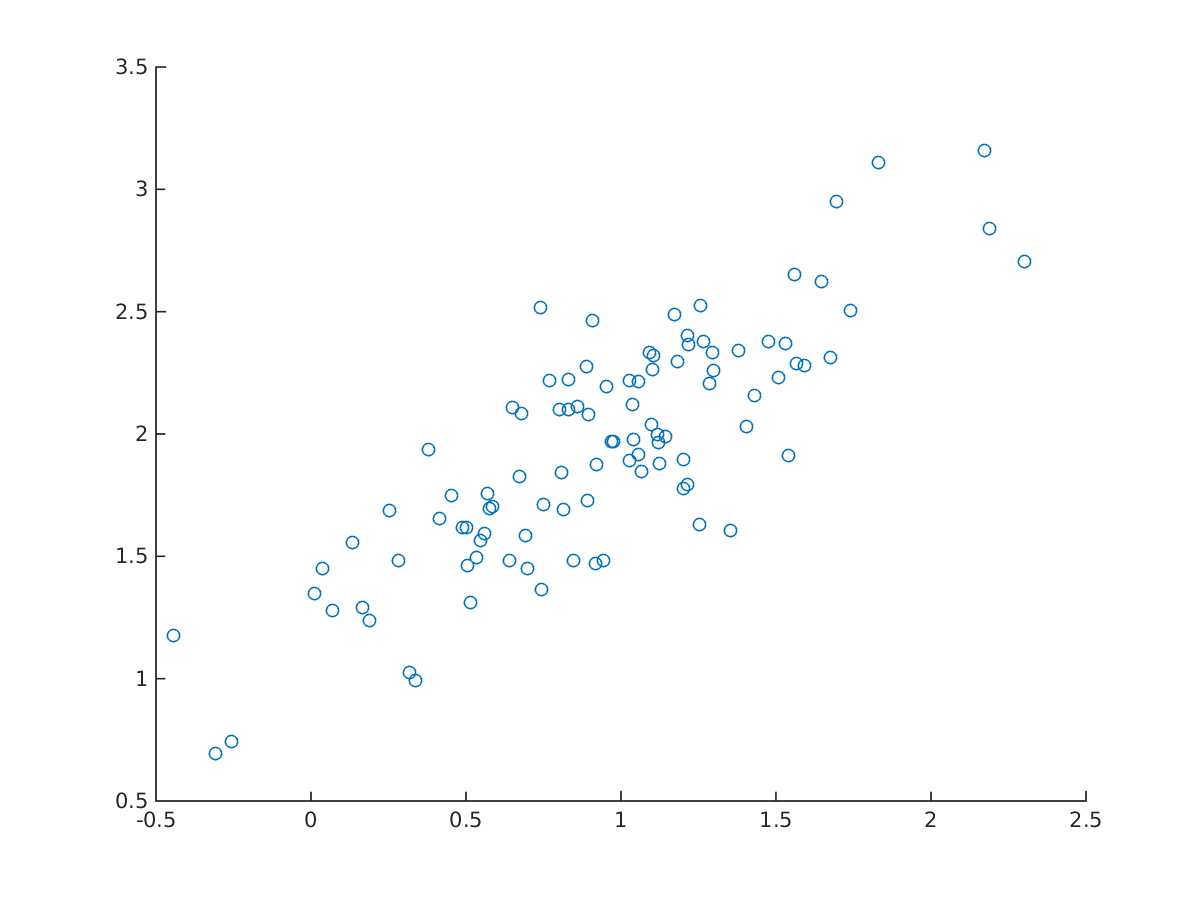
\includegraphics[width=\textwidth]{part1/I222.png}
        \caption{Sample distribution with (\ref{eq:2.2mean}) and (\ref{eq:2.2co})}
    \end{subfigure}
    \caption{Gaussian distribution with varying parameters}
    \label{fig:I2.2}
\end{figure}
\subsubsection{Code}

\inputminted{matlab}{part1/i22john.m}

\subsection{I2.3}


We calculated the mean of the dataset and plotted it ontop of the sampled
data together with the "actual" mean (1,2) as seen in \ref{fig:I3.1}

\begin{figure}[!ht]
    \centering
    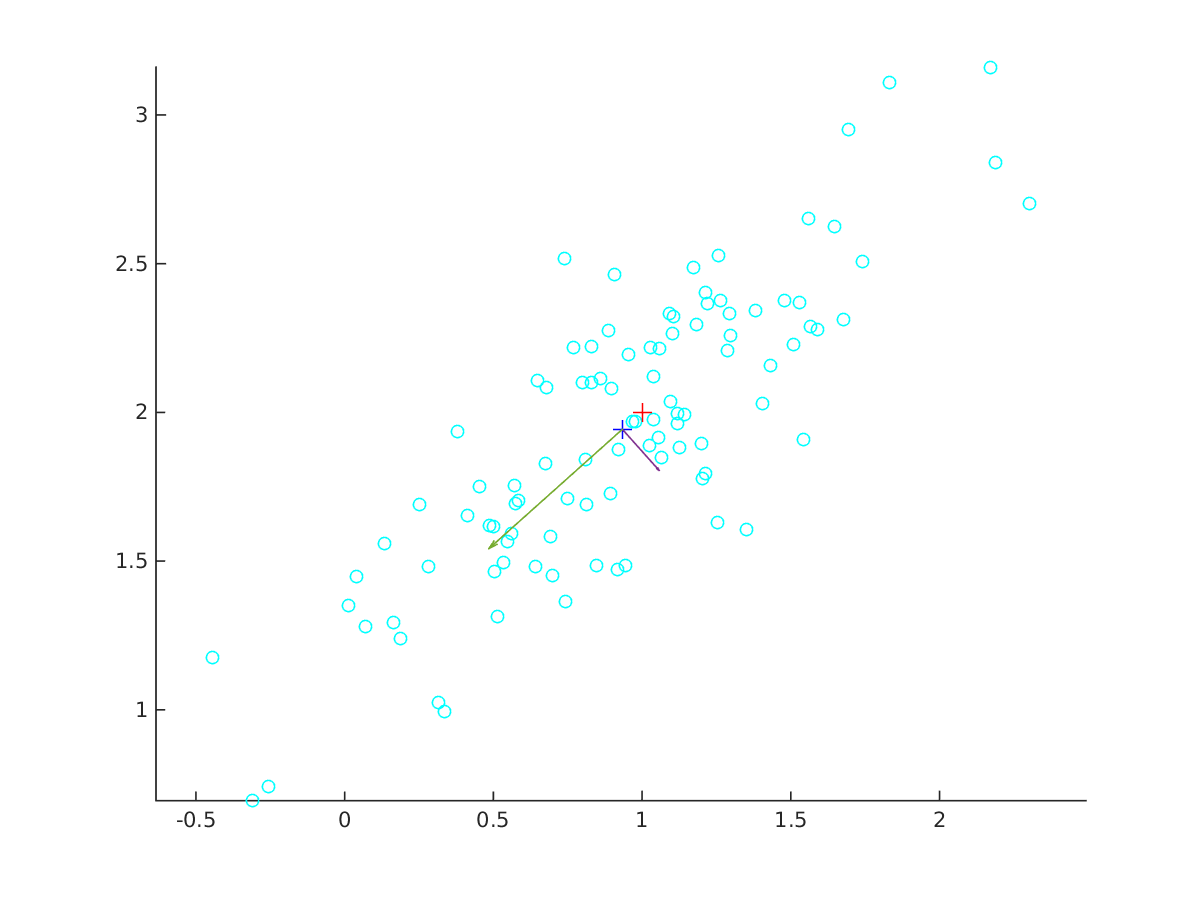
\includegraphics[width=\textwidth]{part1/I231.png}
    \caption{The dataset with the sample mean plotted as a blue '+' and
    distribution mean as a red '+'. The two eigenvectors are also plotted.}
    \label{fig:I3.1}
\end{figure}

The two points deviate because the sample is drawn from a random
distribution which does not necessarily give a sample balanced around the
mean of the distribution. As the amount of datapoints in the sample
increase, the mean should approach the distribution mean.

\subsubsection{Code}

\inputminted{matlab}{part1/i23john.m}

\subsection{I2.4}

The eigenvectors are plotted in figure \ref{fig:I3.1} and describe in which
directions the sample spreads and the eigenvalues describe how heavily it
spreads in the respective direction.

\begin{figure}[!ht]
    \centering
    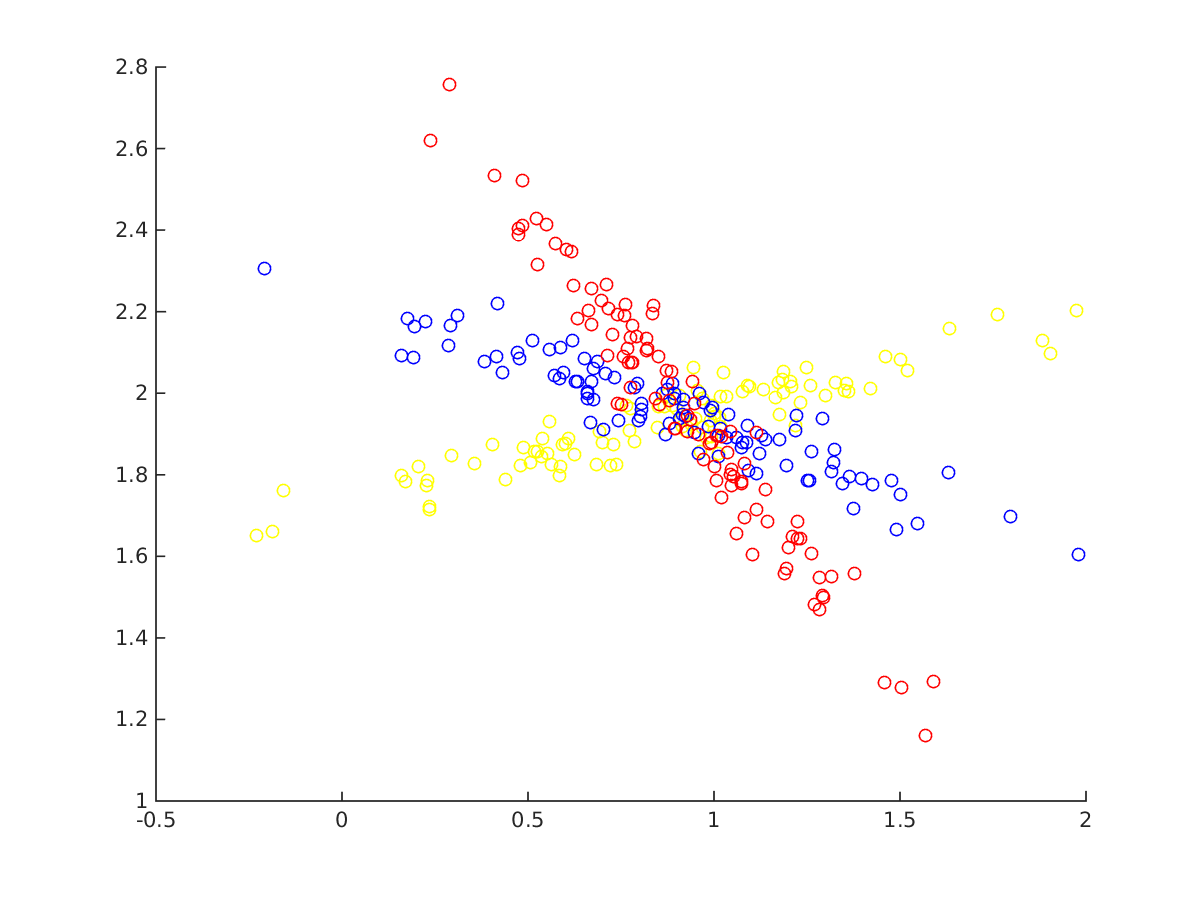
\includegraphics[width=\textwidth]{part1/I241.png}
    \caption{Three different rotations of the sample. The yellow one is
    rotated 30 degrees, the blue one 60 and the red 90.}
    \label{fig:I4.1}
\end{figure}

\begin{figure}[!ht]
    \centering
    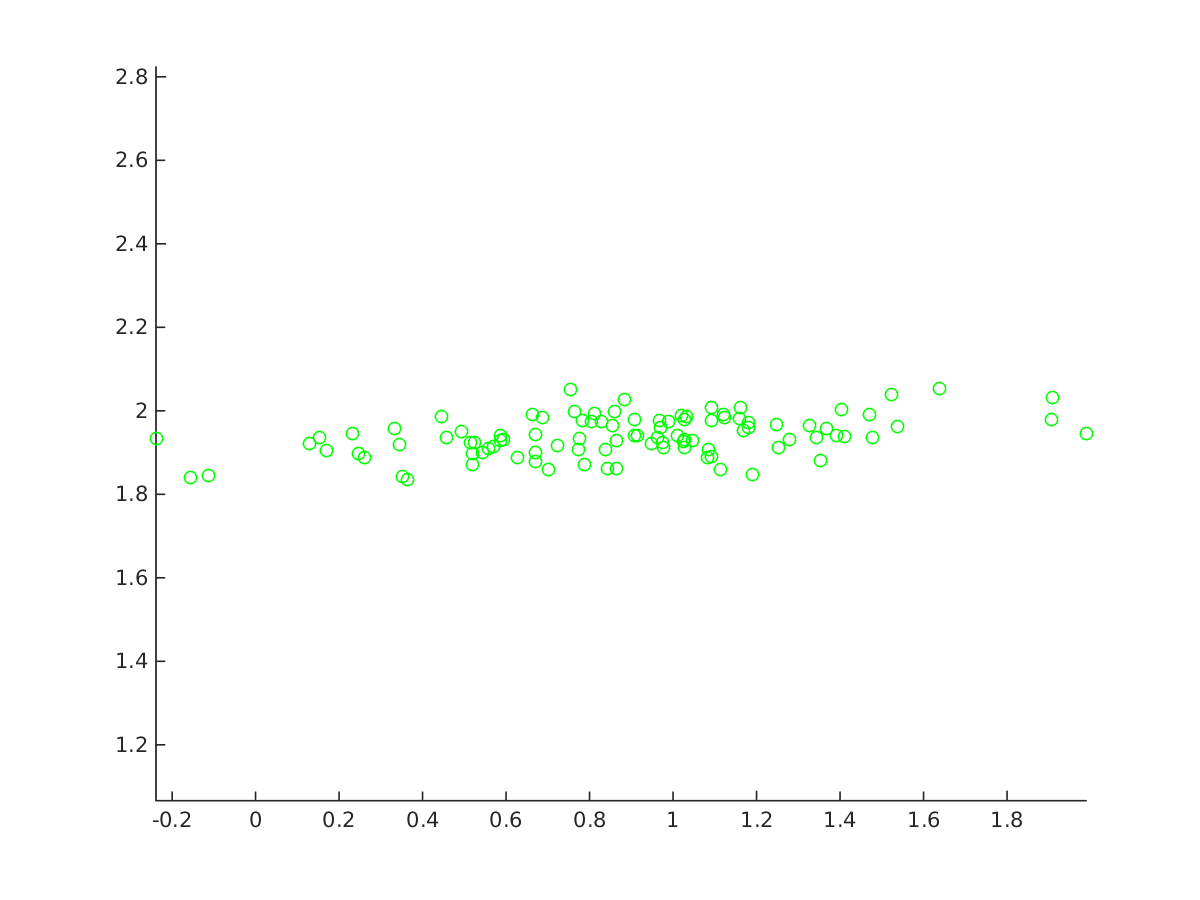
\includegraphics[width=\textwidth]{part1/I242.png}
    \caption{The sample rotated 40 degrees.}
    \label{fig:I4.2}
\end{figure}

The rotated samples are plotted in figure \ref{fig:I4.1}. As seen in
figure \ref{fig:I4.2} is looks likes a rotation of 40 degrees will just
about tilt it to lie parallel to the x-axis.



\subsubsection{Code}

\inputminted{matlab}{part1/i24john.m}


\section{I.3}

The code for all the following assignments can be found in the appendix.

\subsection{I.3.1}
We ran the code and got the following results from $k = \{1,3,5\}$\\
\subsubsection*{Results}
Hit ratio with 1 was {\color{green}81.5789473684\%}. With 38.0 tries 31.0 hits and 7.0 misses\\
Hit ratio with 3 was {\color{yellow}68.4210526316\%}. With 38.0 tries 26.0 hits and 12.0 misses\\
Hit ratio with 5 was {\color{yellow}60.5263157895\%}. With 38.0 tries 23.0 hits and 15.0 misses\\
Where k = 1 is clearly the best classifier.\\

\subsection{I.3.2i}

The cross-validation was done by splitting the test collection into
5 equal sizes, and running the code 5 times with one fifth of the full
collection as the test data and the rest as the training.\\\\ The code
was run as cross-validation with k-values ranging from 1 to 25 and the
data was not normalized. We chose to include the even numbers.

 \subsubsection*{Results}
Average result:\\ 
Hit ratio with 1 was {\color{green}77.75\%}. With 80 tries 62.2 hits and 17.8 misses\\
Hit ratio with 2 was {\color{green}73.5\%}. With 80 tries 58.8 hits and 21.2 misses\\
Hit ratio with 3 was {\color{green}74.0\%}. With 80 tries 59.2 hits and 20.8 misses\\
Hit ratio with 4 was {\color{green}72.5\%}. With 80 tries 58.0 hits and 22.0 misses\\
Hit ratio with 5 was {\color{yellow}67.0\%}. With 80 tries 53.6 hits and 26.4 misses    \\
Hit ratio with 6 was {\color{yellow}67.25\%}. With 80 tries 53.8 hits and 26.2 misses   \\
Hit ratio with 7 was {\color{green}70.75\%}. With 80 tries 56.6 hits and 23.4 misses    \\
Hit ratio with 8 was {\color{green}74.25\%}. With 80 tries 59.4 hits and 20.6 misses  \\  
Hit ratio with 9 was {\color{red}56.75\%}. With 80 tries 45.4 hits and 34.6 misses  \\
Hit ratio with 10 was {\color{red}56.0\%}. With 80 tries 44.8 hits and 35.2 misses  \\
Hit ratio with 11 was {\color{yellow}62.5\%}. With 80 tries 50.0 hits and 30.0 misses   \\
Hit ratio with 12 was {\color{red}54.25\%}. With 80 tries 43.4 hits and 36.6 misses     \\
Hit ratio with 13 was {\color{red}51.0\%}. With 80 tries 40.8 hits and 39.2 misses    \\  
Hit ratio with 14 was {\color{red}48.75\%}. With 80 tries 39.0 hits and 41.0 misses \\
Hit ratio with 15 was {\color{red}48.0\%}. With 80 tries 38.4 hits and 41.6 misses  \\
Hit ratio with 16 was {\color{red}43.0\%}. With 80 tries 34.4 hits and 45.6 misses  \\
Hit ratio with 17 was {\color{red}38.75\%}. With 80 tries 31.0 hits and 49.0 misses \\
Hit ratio with 18 was {\color{red}39.5\%}. With 80 tries 31.6 hits and 48.4 misses  \\
Hit ratio with 19 was {\color{red}35.0\%}. With 80 tries 28.0 hits and 52.0 misses  \\
Hit ratio with 20 was {\color{red}32.0\%}. With 80 tries 25.6 hits and 54.4 misses  \\
Hit ratio with 21 was {\color{red}32.0\%}. With 80 tries 25.6 hits and 54.4 misses  \\
Hit ratio with 22 was {\color{red}32.0\%}. With 80 tries 25.6 hits and 54.4 misses  \\
Hit ratio with 23 was {\color{red}32.0\%}. With 80 tries 25.6 hits and 54.4 misses  \\
Hit ratio with 24 was {\color{red}32.0\%}. With 80 tries 25.6 hits and 54.4 misses  \\
Hit ratio with 25 was {\color{red}32.0\%}. With 80 tries 25.6 hits and 54.4 misses  \\
The best ratio was: 77.75 with a k value of 1\\\\
Without normalizing the data, the k-value with the best result between the 5 runs was the one with a k of 1, with 8 being secondbest.\\
k = 1 had an average miss rate of 17.8.

\subsection{I.3.3}


\subsubsection*{Results}


\newpage
\begin{appendices}

\section{Code for I.2}

\inputminted{matlab}{matlab.m}

\section{Code for I.3}

\inputminted{python}{part2/neighborJohn.py}

\end{appendices}

\end{document}
